\section{Monad}
Now we come to the module \verb\Monad\.
This module takes a mathematical concept and makes into practical programming construct.

First we are going to look at what monads exactly are within programming.
Then we will see how they are implemented within MC.

\subsection{Monads}
Monads are a container like, generic interface.
They contain two functions:

\begin{itemize}
   \item Return
   \item Bind
\end{itemize}

These two functions create the basis on which the monads are built.

\subsubsection{Return}
The return function takes a value and wraps it inside a monad.

{
   \centering
   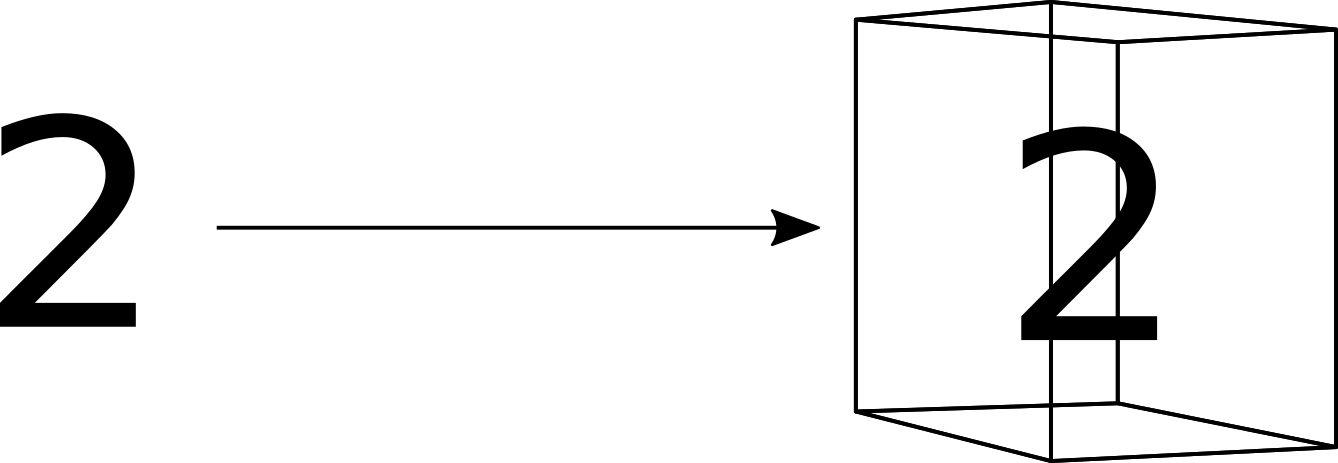
\includegraphics[width=\columnwidth]{return}\\
   \captionof{figure}{The return}\label{fig:monadreturn}
}

The box in figure~\ref{fig:monadreturn} visualizes the monad and \verb\2\ is the value that is being put inside the monad.
With the return function any value can be put inside a monad.
When it is inside the monad it cannot be seen by the outside world.

This is where the bind comes in.

\subsubsection{Bind}
Having a monad is fine, but what if you want to manupilate the value of the monad?
The bind function supplies this functionality.

{
   \centering
   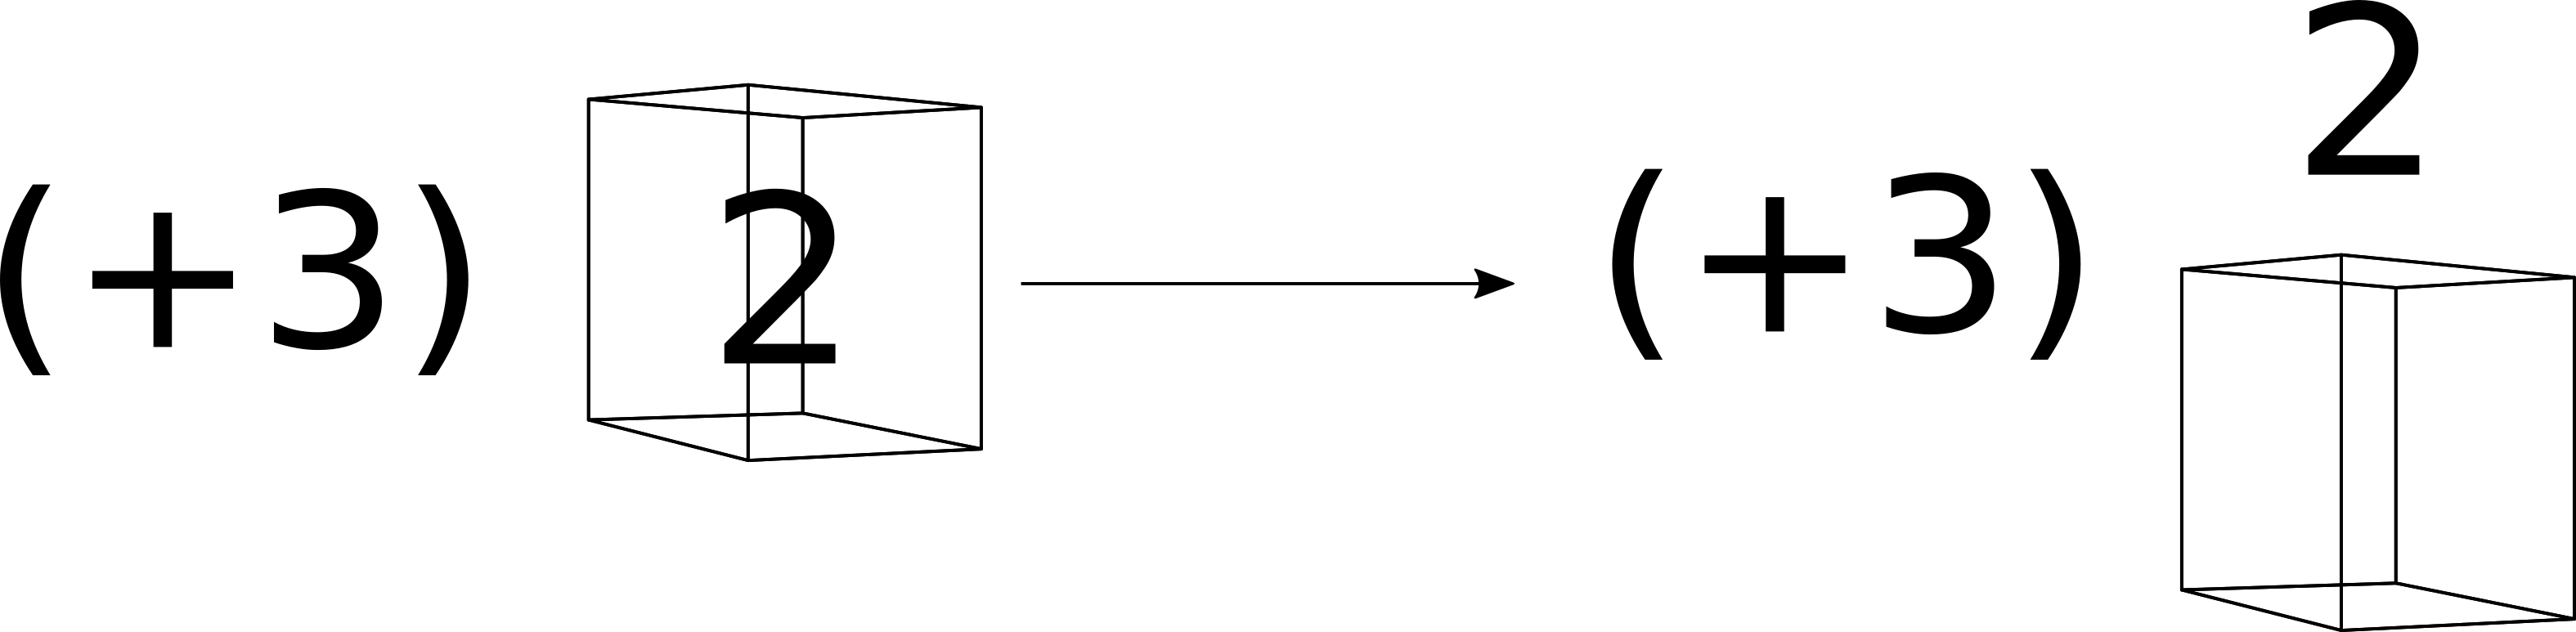
\includegraphics[width=\columnwidth]{bind1}\\
   \captionof{figure}{A function and a monad}\label{fig:monadreturn}
}

When we want to apply the function \verb\(+3)\ to the monad containing \verb\2\, we call the bind.
The bind unpacks the monad.

{
   \centering
   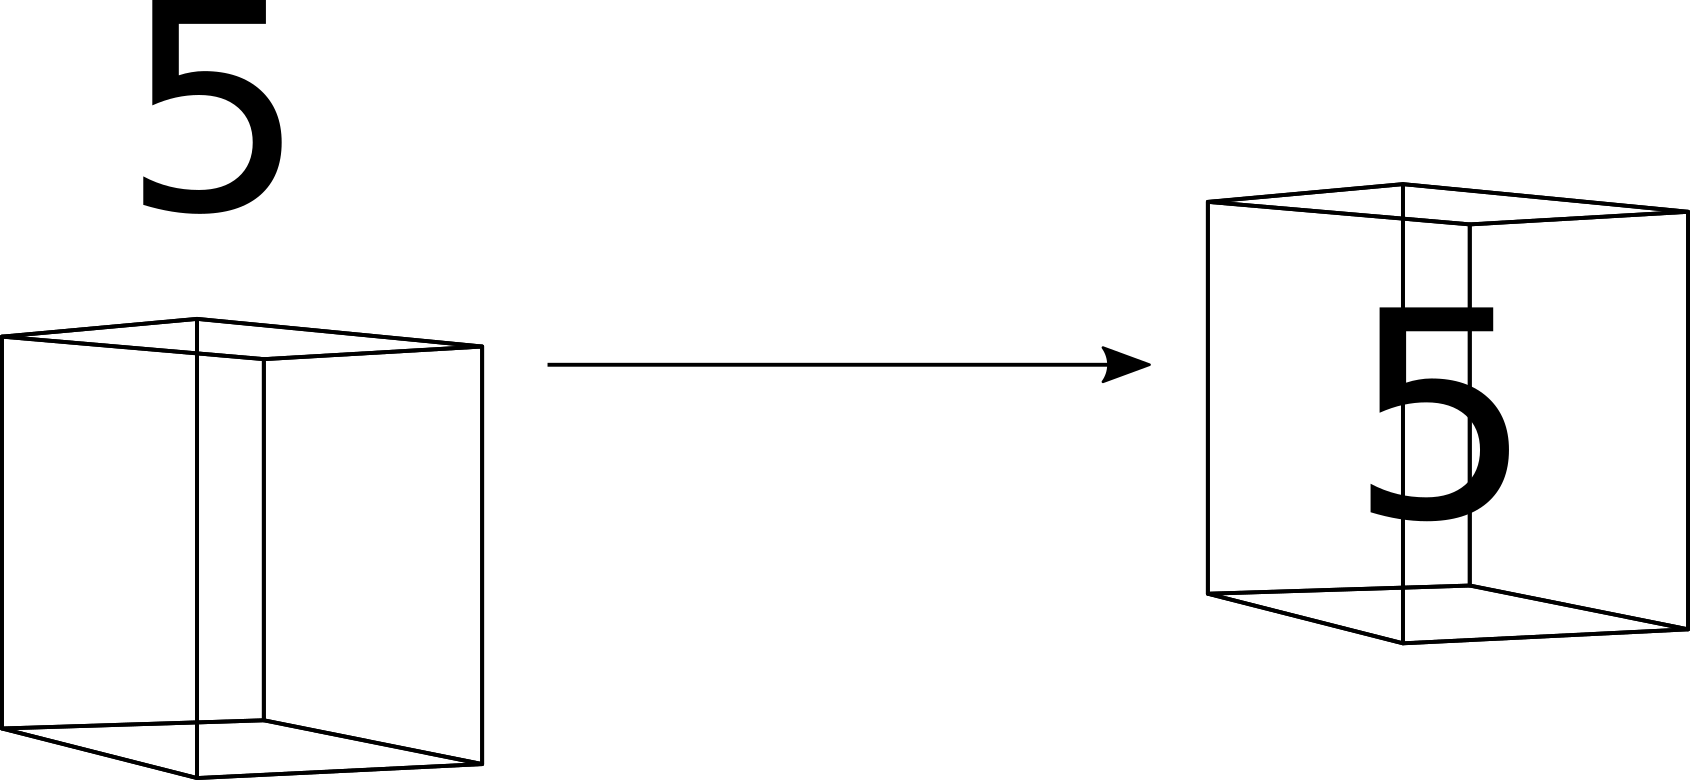
\includegraphics[width=\columnwidth]{bind2}\\
   \captionof{figure}{The return}\label{fig:monadreturn}
}

Applies the function to the value.
And then packs the new value inside the monad.

This way we can work with the safety of the monads, while having the ability to do computations with them.

Different Monads
\begin{itemize}
   \item State
   \item Maybe
\end{itemize}

Parser monad $\Longrightarrow$ State monad $\longrightarrow$ Maybe Monad \\
\vspace{\baselineskip}

Combining Monads:\\
\begin{itemize}
   \item By hand
   \item Error prone
\end{itemize}


{
   \centering
   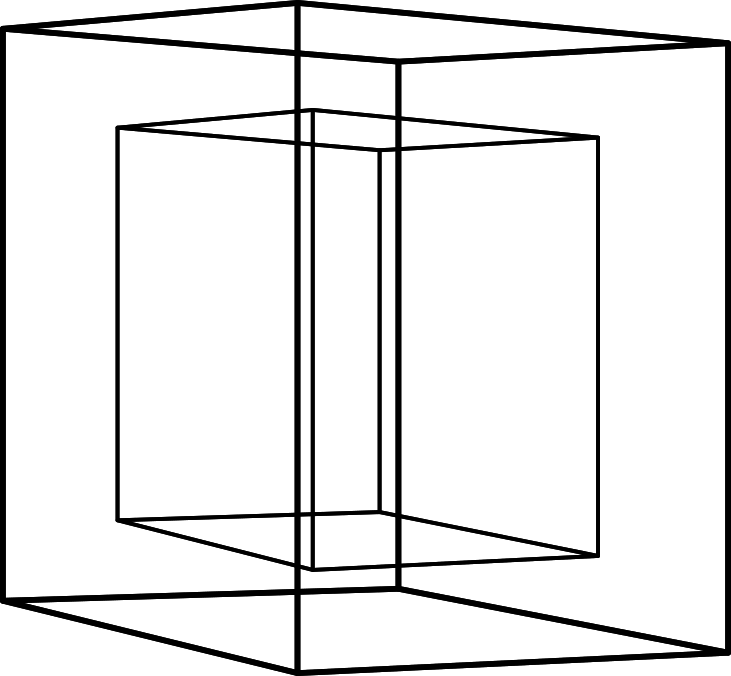
\includegraphics{transformers}\\
   \captionof{figure}{The return}\label{fig:monadreturn}
}

\begin{itemize}
   \item Automatically combines monads
   \item Id monad
\end{itemize}

Id monad
\begin{lstlisting}
TypeAlias "Id" => #a => #b
Id 'a => 'a

TypeFunc "id" => Monad
id => Monad(Id) {
   bind x k -> k x
      return x -> x
}
\end{lstlisting}

\subsubsection{Monad transformers}
\subsection{Implementation}
\subsection{Evolution}

\section{TryableMonad}
\subsection{Evolution}

\section{Implemented monads}
\subsection{Id}
\subsubsection{Evolution}
\subsection{List}
\subsubsection{Evolution}
\subsection{Either}
\subsubsection{Evolution}
\subsection{Option}
\subsubsection{Evolution}
\subsection{Result}
\subsubsection{Evolution}
\subsection{State}
\subsubsection{Evolution}
\subsection{IO}
\subsubsection{Evolution}
